% This is "aamas2014.tex", a revised version of aamas2013.tex
% This file should be compiled with "aamas2014.cls" 
% This example file demonstrates the use of the 'aamas2014.cls'
% LaTeX2e document class file. It is for those submitting
% articles to AAMAS 2014  conference. This file is based on
% the sig-alternate.tex example file.
% The 'sig-alternate.cls' file of ACM will produce a similar-looking,
% albeit, 'tighter' paper resulting in, invariably, fewer pages.
% than the original style ACM style.
%
% ----------------------------------------------------------------------------------------------------------------
% This .tex file (and associated .cls ) produces:
%       1) The Permission Statement
%       2) The Conference (location) Info information
%       3) The Copyright Line with AAMAS data
%       4) NO page numbers
%
% as against the acm_proc_article-sp.cls file which
% DOES NOT produce 1) through 3) above.
%
% Using 'aamas2014.cls' you don't have control
% from within the source .tex file, over both the CopyrightYear
% (defaulted to 200X) and the IFAAMAS Copyright Data
% (defaulted to X-XXXXX-XX-X/XX/XX).
% These information will be overwritten by fixed AAMAS 2014  information
% in the style files - it is NOT as you are used with ACM style files.
%
% ---------------------------------------------------------------------------------------------------------------
% This .tex source is an example which *does* use
% the .bib file (from which the .bbl file % is produced).
% REMEMBER HOWEVER: After having produced the .bbl file,
% and prior to final submission, you *NEED* to 'insert'
% your .bbl file into your source .tex file so as to provide
% ONE 'self-contained' source file.
%

% This is the document class for full camera ready papers and extended abstracts repsectively 

\documentclass{aamas2014_extendedabstract}
\usepackage{times,helvet,courier}
\usepackage{amssymb,amsmath,latexsym}
\usepackage{graphics,graphicx}
\usepackage{subfigure}
\usepackage{algorithm}
\usepackage{algorithmic}
\usepackage{paralist}
\usepackage{layout}
\usepackage{url}
\usepackage{mathptmx} % assumes new font selection scheme installed
\usepackage{epsfig} % for postscript graphics files
\usepackage{pdfsync}
\usepackage{subfigure}



%%%%%%%%%%%%%%%%%%%%%%%%%%%%%%%%%%%%%%%%%%%%%%%%%%%%%%%%%%%%%%%%%%%%%%
%%% Definitions
%%%%%%%%%%%%%%%%%%%%%%%%%%%%%%%%%%%%%%%%%%%%%%%%%%%%%%%%%%%%%%%%%%%%%%

\newcommand{\veh}{\ensuremath{v}}

% \newcommand{\vin}{\textsf{id}}
% \newcommand{\Anchor}{\textsf{Anchor}}



%%%%%%%%%%%%%%%%%%%%%%%%%%%%%%%%%%%%%%%%%%%%%%%%%%%%%%%%%%%%%%%%%%%%%%
%%% Helper functions
%%%%%%%%%%%%%%%%%%%%%%%%%%%%%%%%%%%%%%%%%%%%%%%%%%%%%%%%%%%%%%%%%%%%%%

\newenvironment{small_ind_s_itemize}{\begin{list}{$\bullet$}
{\setlength{\rightmargin}{0em}
\setlength{\leftmargin}{1em}
\setlength{\itemsep}{0em}
\setlength{\topsep}{0em}
\setlength{\parsep}{0em}}}{\end{list}}

\newtheorem{defn}{Definition}          % definition
\newtheorem{thm}{Theorem}              % theorem

\newcommand{\commentc}[1]{{\bf **Chiu: #1**}}
\newcommand{\commentn}[1]{{\bf **Shun: #1**}}
\newcommand{\commentp}[1]{{\bf **Peter: #1**}}


% The following packages can be found on http:\\www.ctan.org
%\usepackage{graphics} % for pdf, bitmapped graphics files
%\usepackage{epsfig} % for postscript graphics files
%\usepackage{mathptmx} % assumes new font selection scheme installed
%\usepackage{times} % assumes new font selection scheme installed
%\usepackage{amsmath} % assumes amsmath package installed
%\usepackage{amssymb}  % assumes amsmath package installed

\begin{document}

% \setlength\titlebox{1.8in}


\title{Semi-Autonomous Intersection Management}

%\author{ \parbox{3 in}{\centering Huibert Kwakernaak*
%         \thanks{*Use the $\backslash$thanks command to put information here}\\
%         Faculty of Electrical Engineering, Mathematics and Computer Science\\
%         University of Twente\\
%         7500 AE Enschede, The Netherlands\\
%         {\tt\small h.kwakernaak@autsubmit.com}}
%         \hspace*{ 0.5 in}
%         \parbox{3 in}{ \centering Pradeep Misra**
%         \thanks{**The footnote marks may be inserted manually}\\
%        Department of Electrical Engineering \\
%         Wright State University\\
%         Dayton, OH 45435, USA\\
%         {\tt\small pmisra@cs.wright.edu}}
%}

\numberofauthors{1}
\author{
% You can go ahead and credit any number of authors here,
% e.g. one 'row of three' or two rows (consisting of one row of three
% and a second row of one, two or three).
%
% The command \alignauthor (no curly braces needed) should
% precede each author name, affiliation/snail-mail address and
% e-mail address. Additionally, tag each line of
% affiliation/address with \affaddr, and tag the
% e-mail address with \email.
% 1st. author
\alignauthor
Paper ID: 279
%Ben Trovato\titlenote{Dr.~Trovato insisted his name be first.}\\
%       \affaddr{Institute for Clarity in Documentation}\\
%       \affaddr{1932 Wallamaloo Lane}\\
%       \affaddr{Wallamaloo, New Zealand}\\
%       \email{trovato@corporation.com}
% 2nd. author
%\alignauthor
%G.K.M. Tobin\titlenote{The secretary disavows any knowledge of this author's actions.}\\
%       \affaddr{Institute for Clarity in Documentation}\\
%       \affaddr{P.O. Box 1212}\\
%       \affaddr{Dublin, Ohio 43017-6221}\\
%       \email{webmaster@marysville-ohio.com}
% 3rd. author
%\alignauthor Lars Th{\o}rv{\"a}ld\titlenote{This author is the one who did all the really hard work.}\\
%       \affaddr{The Th{\o}rv{\"a}ld Group}\\
%       \affaddr{1 Th{\o}rv{\"a}ld Circle}\\
%       \affaddr{Hekla, Iceland}\\
%       \email{larst@affiliation.org}
}


% \author{Tsz-Chiu Au, Shun Zhang and Peter Stone}

% \author{Huibert Kwakernaak$^{1}$ and Pradeep Misra$^{2}$% <-this % stops a space
% \thanks{*This work was not supported by any organization}% <-this % stops a space
% \thanks{$^{1}$H. Kwakernaak is with Faculty of Electrical Engineering, Mathematics and Computer Science,
%         University of Twente, 7500 AE Enschede, The Netherlands
%         {\tt\small h.kwakernaak at papercept.net}}%
% \thanks{$^{2}$P. Misra is with the Department of Electrical Engineering, Wright State University,
%         Dayton, OH 45435, USA
%         {\tt\small p.misra at ieee.org}}%
% }




\maketitle

\thispagestyle{empty}
\pagestyle{empty}


%%%%%%%%%%%%%%%%%%%%%%%%%%%%%%%%%%%%%%%%%%%%%%%%%%%%%%%%%%%%%%%%%%%%%%%
% Abstract
%%%%%%%%%%%%%%%%%%%%%%%%%%%%%%%%%%%%%%%%%%%%%%%%%%%%%%%%%%%%%%%%%%%%%%%

\begin{abstract}
Autonomous Intersection Management
(AIM) is a reservation-based intersection control protocol that
leverages the capacities of autonomous vehicles to dramatically reduce
traffic delay at intersections. AIM was designed for the time when
all, or most, of the vehicles on the road are \emph{fully} autonomous.
However, we anticipate that there will be a long transition
period during which many cars are still driven by human drivers and/or
most vehicles have some but not all capabilities of fully autonomous
vehicles. In order to accommodate this transition, this paper
introduces a new multiagent protocol called \emph{Semi-Autonomous
Intersection Management} (SemiAIM), which allows vehicles with
partially-autonomous features such as adaptive cruise control to make
reservations in AIM\@.  We propose a method for vehicles with limited
autonomy to make reservations to enter an intersection in an AIM-like
style and conduct extensive experiments in simulation to evaluate its
effectiveness.  Our results show that the delay of semi-autonomous
vehicles in SemiAIM can be greatly reduced compared to human-driven
vehicles.
\end{abstract}


% In fact, this transition period has already begun---adaptive cruise
% control systems and lane departure warning systems have become widely
% available as optional equipment on luxury production vehicles since
% the late 1990s.



% Note that the category section should be completed after reference to the ACM Computing Classification Scheme available at
% http://www.acm.org/about/class/1998/.

\category{I.2.11}{Artificial Intelligence}{Distributed Artificial Intelligence---Multiagent systems}
\vspace{-.05in}

% \category{H.4}{Information Systems Applications}{Miscellaneous}

%A category including the fourth, optional field follows...
%\category{D.2.8}{Software Engineering}{Metrics}[complexity measures, performance measures]

%General terms should be selected from the following 16 terms: Algorithms, Management, Measurement, Documentation, Performance, Design, Economics, Reliability, Experimentation, Security, Human Factors, Standardization, Languages, Theory, Legal Aspects, Verification.

\terms{Algorithms, Performance, Economics, Experimentation, Theory}
\vspace{-.05in}

% \terms{Delphi theory}

%Keywords are your own choice of terms you would like the paper to be indexed by.

\keywords{Autonomous vehicles, multiagent systems, coordination}

% \keywords{AAMAS proceedings, \LaTeX, text tagging}



%%%%%%%%%%%%%%%%%%%%%%%%%%%%%%%%%%%%%%%%%%%%%%%%%%%%%%%%%%%%%%%%%%%%%%%
% Contents
%%%%%%%%%%%%%%%%%%%%%%%%%%%%%%%%%%%%%%%%%%%%%%%%%%%%%%%%%%%%%%%%%%%%%%%

\sloppy
\section{Introduction}
\label{sec:introduction}

Recent robotic car competitions and demonstrations have convincingly
shown that autonomous vehicles are feasible with the current
generation of hardware~\cite{mybib:Darpa07Urban}. Looking ahead to the
time when autonomous cars will be common, Dresner and Stone proposed a
new intersection control protocol called \emph{Autonomous Intersection
Management} (AIM) and showed that by leveraging the control and
network capabilities of autonomous vehicles it is possible to design
an intersection control protocol that is much more efficient than
traffic signals~\cite{bib:Dresner08Multiagent}.  By removing human
factors from control loops, autonomous vehicles, with the help of
advanced sensing devices, can be safer and more reliable than human
drivers.  The AIM protocol exploits the fine control of autonomous
vehicles to allow more vehicles simultaneously to cross an
intersection, thus effectively reducing the delay of vehicles by
orders of magnitude compared to traffic
signals~\cite{bib:Fajardo12Automated}.

AIM is designed for the time when vehicles are autonomous.  We,
however, anticipate that there will be a long transition period during
which most vehicles have some but not all capabilities of fully
autonomous vehicles.  In fact, this transition period has already
begun. Since the late 1990s, adaptive cruise control systems and lane
departure warning systems have become widely available as optional
equipment on luxury production vehicles.  Today's automatic parking
systems such as those in the Toyota Prius and various BMW models can
perform parallel parking with little or no human intervention.  While
AIM provides a significant efficiency improvement at intersections
when all cars are autonomous, the benefits are minimal even when as
few as 10\% of the vehicles are driven by humans (Figure 16
in~\cite{bib:Dresner08Multiagent}).  The requirement that most,
if not all,
vehicles are fully autonomous is a key obstacle to the adoption
of AIM-like intersection control when most vehicles are not fully autonomous.

% The National Highway Traffic Safety Administration acknowledges that
% fully autonomous vehicles represent just the top level in five levels
% of vehicle automation~\cite{bib:NHTSA13Preliminary}. Indeed, they
% define a level below this top level with vehicles that
% have limited self-driving automation.
% The main motivation of this paper is to
% propose a new intersection control system called
% \emph{Semi-Autonomous Intersection Management (SemiAIM)} that can
% accomodate both fully autonomous vehicles and
% \emph{semi-autonomous} vehicles with limited self-driving automation.
% There is a high likelihood that
% human-driven vehicles, semi-autonomous vehicles, and fully autonomous
% vehicles will \emph{coexist} on the road in the future.  SemiAIM takes
% advantages of this trend and allows autonomous intersections to handle
% a traffic mixture with different types of vehicles.
% 
% The main contributions of this paper are 1) the introduction of the
% concept of SemiAIM; 2) a full specification of the reservation
% requests for SemiAIM; and 3) detailed empirical results demonstrating
% the effectiveness of this protocol, especially in moderate traffic
% levels with a mix of human-driven, semi-autonomous, and fully
% autonomous vehicles.  The remainder of the paper is organized as
% follows.  Section~\ref{sec:aim} outlines the architecture of AIM which
% forms the basis of SemiAIM.  Section~\ref{sec:vehicles} categorizes
% semi-autonomous vehicles that work with SemiAIM.
% Section~\ref{sec:interface} discusses the design of the user interface
% for drivers on semi-autonomous vehicles to interact with SemiAIM.
% Section~\ref{sec:constraint} describes the constraint-based
% reservation system, a generalization of AIM for semi-autonomous
% vehicles.  Section~\ref{sec:simulation} presents the results of the
% simulation experiments we used to evaluates SemiAIM.  The related work
% and the conclusion are given in Section~\ref{sec:related} and
% \ref{sec:conclusions}, respectively.
% 

% In this paper, semi-autonomous vehicles meet the criteria of limited
% self-driving automation (Level 3).
% Another motivation for SemiAim is the drawback of AIM.  

% The main motivation for SemiAim is that we anticipate that there will
% be a long transition period during which most vehicles have some but
% not all capabilities of fully autonomous vehicles.  In fact, this
% transition period has already begun. Since the late 1990s, adaptive
% cruise control systems and lane departure warning systems have become
% widely available as optional equipment on luxury production vehicles.
% Today's automatic parking systems such as those in the Toyota Prius
% and various BMW models can perform parallel parking with little or no
% human intervention. The National Highway Traffic Safety Administration
% defines five levels of vehicle automation~\cite{NHTSA2013}. In this
% paper, semi-autonomous vehicles meet the criteria of limited
% self-driving automation (Level 3). Fully autonomous vehicles are
% equivalent with full self-driving automation (Level 4).  Hence, there
% is an opportunity to develop an intersection control protocol that
% works with these semi-autonomous vehicles.  More importantly, there is
% a high likelihood that human-driven vehicles, semi-autonomous
% vehicles, and fully autonomous vehicles will \emph{coexist} on the
% road in the future.  SemiAIM takes advantages of this trend and allows
% autonomous intersections to handle a traffic mixture with different
% types of vehicles.

% Another motivation for SemiAim is the drawback of AIM.  The AIM policy
% has a significant improvement on the efficiency of intersection, but
% that requires the ratio of fully autonomous vehicles exceed 95\% of
% all type of vehicles. Even if the ratio of fully autonomous vehicles
% exceeds 90\%, there is no significant difference from traffic signal
% policy (Figure 16 in~\cite{bib:Dresner08Multiagent}). 




% In this paper, we introduce a new protocol called
% \emph{Semi-Autonomous Intersection Management} (SemiAIM), which allows
% vehicles with partially-autonomous features such as adaptive cruise
% control to make reservations in AIM.  We demonstrate the feasibility
% for vehicles with limited autonomy to make reservations to enter an
% intersection in AIM-like style.  Our simulation results show that
% traffic delay of semi-autonomous vehicles in SemiAIM is nearly as
% small as the traffic delay of fully-autonomous vehicles in AIM.


% The paper starts with a discussion of the need of a traffic system
% that can handle autonomous, semi-autonomous, and manual-controlled
% vehicles.  Then we discuss the previous work of FCFS-signals and its
% weaknesses.  Then we propose a new AIM-like reservation systems that
% allow human compatible reservation requests.

% Perhaps, with the help of a cellphone, it can send request.
% For example, if the human driver is maintaining a constant speed,
% it will then send the request. If he receive a confirmation
% and believe that the vehicle can continue to maintain the speed,
% it can go through the intersection without stopping.


%%% Local Variables: 
%%% mode: latex
%%% TeX-master: "main"
%%% End:

%\section{Autonomous Intersection Management}
\label{sec:aim}

The AIM protocol is based on a \emph{reservation} paradigm, in which
vehicles ``call ahead'' to reserve space-time in the
intersection~\cite{bib:Dresner08Multiagent}. The system assumes that
computer programs called \emph{driver agents} control the vehicles,
while an arbiter agent called an \emph{intersection manager} (IM) is
placed at each intersection.  The driver agents attempt to reserve a
block of space-time in the intersection.  The intersection manager
decides whether to grant or reject requested reservations according to
an \emph{intersection control policy}.  In brief, the paradigm
proceeds as follows.
\begin{small_ind_s_itemize}
\item An approaching vehicle announces its impending arrival to the
IM.  The vehicle indicates its predicted arrival time, velocity,
acceleration, and arrival and departure lanes.
\item The IM simulates the vehicle's path through
the intersection, checking for conflicts with the paths of any
previously processed vehicles.
\item If there are no conflicts, the IM issues a
reservation. It then becomes the vehicle's responsibility to arrive at, and
travel through, the intersection as specified.
\item The car may only enter the intersection once it has successfully
obtained a reservation.
\end{small_ind_s_itemize}
The prototype intersection control policy called \emph{First Come,
First Served} (FCFS) operates by dividing the intersection into a grid
of \emph{reservation tiles}. When a vehicle approaches the
intersection, the intersection manager uses the data in the
reservation request regarding the time and velocity of arrival,
vehicle size, etc. to simulate the intended journey across the
intersection.  At each simulated time step, the policy determines
which reservation tiles will be occupied by the vehicle.  If the
vehicle's space-time request has no conflict, the reservation is
successful; otherwise, the reservation request will be rejected.

Empirical results in simulation demonstrated that the 
reservation system with FCFS can dramatically improve the intersection
efficiency when compared to traditional intersection control
mechanisms~\cite{bib:Dresner08Multiagent}.  Overall, by
allowing for much finer-grained coordination, the simulation-based
reservation system can dramatically reduce per-car delay by two orders
of magnitude in comparison to traffic signals and stop signs.  This
reduction of delays can translate into less traffic
congestion~\cite{bib:Au10Motion,bib:Quinlan10Bringing}, which in turn
leads to better fuel efficiency and lower emissions.

A drawback of FCFS is that it is designed for fully autonomous
vehicles only---it does not work with any vehicles that require human
operations. If any human-driven vehicle appears. Dresner and Stone did
propose a hybrid protocol called FCFS-Signal (a.k.a. FCFS-Light) which
allows human-driven vehicles to share the road with autonomous
vehicles at intersections~\cite{bib:Dresner07Sharing}. However, their
approach has two major drawbacks.  First, the benefits of FCFS-Signal
over conventional traffic signals are relatively small until 90-95\%
of the vehicles on the road are autonomous.  Second, and most
important for this paper, FCFS-Signal cannot take advantage of the
limited autonomous capabilities of semi-autonomous vehicles. There are
useful features that human-driven vehicles could have, that AIM
managers have overlooked. To remedy these issues, this paper
introduces a new autonomous intersection system called \emph{SemiAIM}
that works not only with autonomous vehicles but also with
human-driven vehicles and semi-autonomous vehicles.


\begin{figure}
\centering
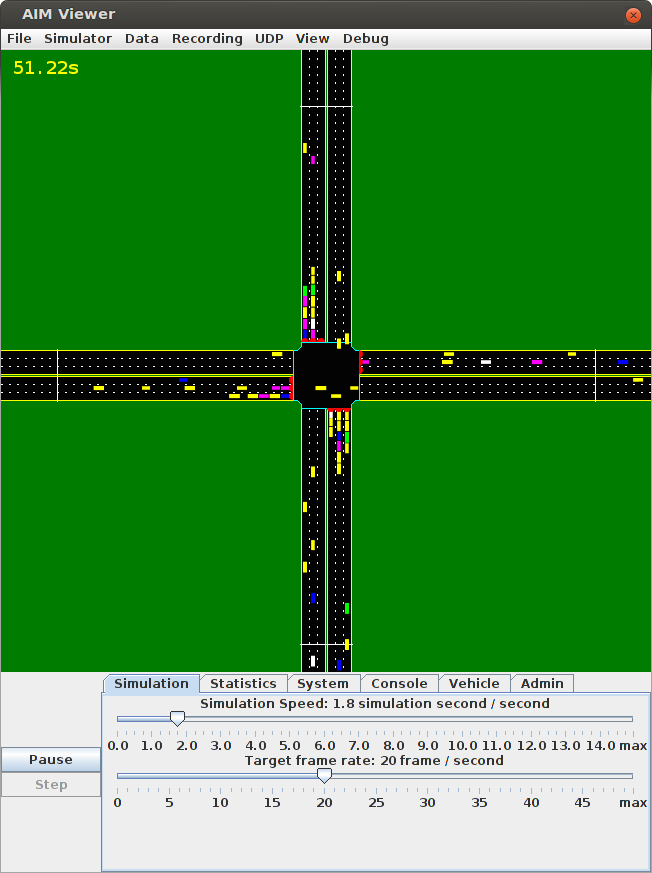
\includegraphics[width=0.8\columnwidth]{figures/demo.png}
\caption{A screenshot of the simulator we developed for the experiments on
SemiAIM.}
\label{fig:simulator}
\end{figure}





% FCFS-Signal (a.k.a. \footnote{It was originally called ``FCFS-Light.''} 


% There are different types of vehicles we'll introduce in
% Section~\ref{sec:vehicles}.


% \commentn {There
% was a paragraph in introduction part describing FCFS-Signal - it was
% called FCFS-light in Dresner's paper. I agree it's better to put it
% here.}



% \commentp{Since we have extra space, there can be a screenshot added
% here.  Also, it would be worthwhile including a description of
% FCFS-signal and describing why that doesn't address the goal of this
% paper (because it assumes that cars are either fully autonomous or
% completely human-controlled).}

%%% Local Variables: 
%%% mode: latex
%%% TeX-master: "gridlock"
%%% End:


\section{Semi-Autonomous Vehicles}
\label{sec:vehicles}

Dresner and Stone proposed the FCFS-signal policy, which makes AIM
compatible with human drivers~\cite{bib:Dresner07Sharing}.  According
to their study, when more than 5-10\% of traffic is comprised of
human-driven vehicles, the average delay time of all vehicles
increases significantly.  For one thing, the human-driven vehicles
themselves may not enter the intersection during red signal phases.
But more importantly, they prevent the autonomous vehicles from
obtaining reservations when they are behind such stalled vehicles.  To
allow more efficient management of traffic at intersections, we
consider human-driven vehicles with additional communication features
to facilitate interaction with the IM and other vehicles. In this
paper, we use the term \emph{semi-autonomous vehicles} to refer to
both the vehicles with simple/adaptive cruise control and human-driven
vehicles with additional communication capabilities. We consider the
following categories of vehicles.

\begin{itemize}

\item \textbf{Autonomous vehicles (Type A).} These are fully
autonomous vehicles that can be totally controlled by computers.

\item \textbf{Semi-autonomous vehicles (Type SA).}
Although they are driven by humans,
they have some devices that can assist human drivers and
can communicate with the IM. In this paper, 
we consider three concrete types of SA vehicles, 
as specified in this section.

\item \textbf{Human-driven vehicles (Type H).}
These vehicles are exactly the same as the ones on today's
roads. They are completely controlled by humans and have no
communication with the IM.

\end{itemize}

Moreover, we classify semi-autonomous vehicles according to the
equipment on the vehicles. We consider the following set of
equipment that can be put on a semi-autonomous vehicle.  This
equipment is based on technology that is readily available today.

\begin{itemize}

\item \textbf{Adaptive cruise control} A vehicle can be set to follow
another vehicle in front of it.  This feature is currently available
as an option in some high-end vehicles. A vehicle with this feature
can propose an \textit{anchor request} that will be discussed in
Section~\ref{sec:request}.  The IM considers whether it can safely
traverse the intersection by following the vehicle in front of it.

\item \textbf{Simple Cruise control} A vehicle can be set to maintain
a constant velocity by turning on cruise control. This is a technology
that is widely available today. A vehicle with this feature can
propose a \textit{constant-velocity request}. The IM considers whether
it can traverse the intersection by keeping a constant velocity.

\item \textbf{Communication device} This is a device, which can be a
smart-phone or on-board navigation system, that can communicate with
the Intersection Manager.  It can gather data from the vehicle, and
communicate instructions to the driver when necessary.  For example,
at a red signal, the IM could inform the driver that it is now safe to
enter the intersection.  A vehicle with such a feature could propose a
\textit{whole-row request} to reserve an entire lane in the
intersection for the vehicle.  This is a very strong request and is
only likely to be confirmed in very light traffic in which an entire
``row'' is available.

% \commentp{As described in Section III? (see next comment), this
%   request is a...}

% \commentp{This is a significant weakness of the paper.  "Whole-row
% request", "constant-velocity request", and "anchor request" haven't
% been defined yet.  They're used below, but really only "anchor
% request" is defined later in the paper (section VI). I think it makes
% more sense to merge section VI into section III and clearly define the
% types of requests that can be defined using constraints.  These
% requests could also be used by fully autonomous vehicles, so there's
% no reason that it needs to happen after section IV.  We can then
% emphasize that the traditional AIM system can also be implemented
% using these constraint-based requests (since a normal "fixed arrival,
% fixed trajectory" request is also possible).}

\end{itemize}

All of this equipment gives semi-autonomous vehicles \emph{some} of
the functionality of autonomous vehicles, even though human drivers
still retain some control of the vehicles.  Next, we introduce several
types of semi-autonomous vehicles that we envision utilizing this
equipment.  For each, we summarize how the semi-autonomous vehicle can
interact with the IM when authorized to do so by the driver.  In
general, having additional equipment provides additional potential
advantages over manually driven cars.  But we emphasize that in all
cases, the human driver can always opt to simply follow the traffic
signals if engaging the equipment is too distracting at any given
time.  Table~\ref{table:type} summarizes the equipment being used on
different types of the semi-autonomous vehicles that we consider.

\begin{table}
\centering
\caption{Features of semi-autonomous vehicles.}
\label{table:type}
\begin{tabular}{|c|c|c|c|}
  \hline
  Vehicle Type & Communication & Cruise & Adaptive \\
               & device & control & cruise control \\
  \hline
  SA-ACC & X & X & X  \\
  \hline
  SA-CC & X & X &  \\
  \hline
  SA-Com & X & &  \\
  \hline
\end{tabular}
\end{table}

\noindent \textbf{Type SA-ACC Vehicles} can utilize all of the above
equipment to make a reservation:
\begin{enumerate}

\item Such a vehicle can propose an anchor request. If the vehicle in
front of it is (semi-)autonomous and is going in the same direction,
then if they can both get reservations, the request is confirmed. The
vehicle can follow the front vehicle and enter the intersection.

\item If the anchor request is denied, it can propose a
constant-velocity request. If keeping the current velocity it can
safely traverse the intersection, the request is confirmed.

\item If the constant-velocity request is denied, it can propose a
whole-row request. If there is no conflict and the vehicle can enter
the intersection directly, the request is confirmed.

\item If denied again, the car must decelerate enough to be able to
stop before the intersection.  It can retry step 3 or pass control to
the human.

\end{enumerate}

\noindent
\textbf{Type SA-CC Vehicles} mainly utilize simple cruise control as follows.
\begin{enumerate}

\item Such a vehicle can propose a constant-velocity request. If it
can enter the intersection by keeping the current velocity, the
request is confirmed.

\item If the constant-velocity request is denied, it can propose a whole-row
  request. If the entire lane is available, the request is confirmed.

\item If denied again, the car must decelerate enough to be able to
stop before the intersection.  It can retry step 2 or pass control to
the human.

\end{enumerate}

\noindent
\textbf{Type SA-Com Vehicles} utilize only communication devices
to make reservations:
\begin{enumerate}

\item Such a vehicle can propose a whole-row request.  If the entire
lane is available, the request is confirmed.

\item If denied again, the car must decelerate enough to be able to
stop before the intersection.  It can retry step 1 or pass control to
the human.

\end{enumerate}

In Figure~\ref{fig:demo}, we color Type A vehicles yellow, Type SA-ACC vehicles
green, Type SA-CC vehicles blue, Type SA-Com vehicles white and Type H
vehicles magenta. The figure shows a red phase for all lanes, Some Type A vehicles
are permitted to enter the intersection.



% Our vehicle types
% SA-ACC, SA-CC, and SA-Com have combinations of these features as
% summarized in 

% Adaptive cruise control
% Used by Type SA-ACC vehicles,

% \item \textbf{Simple Cruise control} (Used by Types SA-ACC and SA-CC
%   vehicles).

% \item \textbf{Communication device} (Used Types SA-ACC, SA-CC, and SA-Com vehicles).



%%% Local Variables: 
%%% mode: latex
%%% TeX-master: "main"
%%% End:

%\section{Interaction Model}
\label{sec:interface}

% In the semi-autonomous vehicles we introduced in the previous section,
% a human driver can always intervene and simply follow the traffic
% signal.

% , as long as no driver runs a red light (without a
% reservation granted).

Safety is a main concern when involving human drivers in the control
loop of semi-autonomous vehicles.  For the semi-autonomous vehicles
defined above to be able to go through an intersection safely, we need
to define a simple and clean interface for negotiating with the IM and
passing control between the human driver and the driver agent.  In
this section, we describe how our proposed protocol can be realized
safely by having an \emph{interaction model} between human drivers and
driver agents that simplifies the task of the human drivers.

Figure~\ref{fig:interaction} summarizes the interaction model between
human drivers, driver agents, and the IM.  We require the inclusion in
the vehicle of a single button that signals the driver agent to ask
for a reservation. After pressing the button, the driver agent will
automatically send a request message to the IM on behalf of the human
driver. It is also important that there is a clear ``Okay'' indicator
(such as a green light) installed in the car which indicates when the
request has been confirmed.  After seeing the okay signal, the driver
would have to actively pass control to the driver agent, again by
pressing a single button.  This way the driver will not be surprised
by any sudden autonomous actions of the vehicle.

\begin{figure*}[t]
\centering
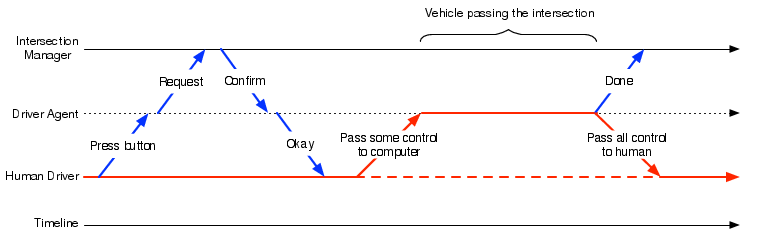
\includegraphics[width=5.5in]{figures/interaction}
\caption{The interaction between human drivers, driver agents, and the
IM.  The blue lines are message passing, and the red lines are
transfer of control.  Note that human drivers retain some control of the vehicle
inside the intersection (the dashed red line).}
\label{fig:interaction}
\vspace{-.1in}
\end{figure*}

This interaction model only requires the human driver to perform
relatively simple driving maneuvers such as holding the steering wheel
at a certain angle (for Types SA-ACC and SA-CC vehicles) or
driving as if under a traffic signal (for Type SA-Com vehicles).
These tasks are much simpler than other maneuvers such as lane
changing and passing other vehicles, and thus should not be taxing to experienced human drivers.  
%Thus it is reasonable to assume
%that human drivers, with enough practice, should manage to perform
%these maneuver perfectly.

% There is a point near the entry of the intersection where it is no
% longer possible to brake before entering the intersection. Beyond this
% point, the person must lose the ability to take back control of the
% speed until leaving the intersection (presumably with an emergency
% override option for extreme situations).  This constraint is based on
% the fact that if the driver were to change its velocity, its
% reservation would need to be modified.  The IM cannot guarantee that
% the modified reservation will be confirmed.

% If the person touches the brakes or accelerator, the person
% regains control, and the reservation is cancelled.


% Two points are important to keep in mind about all the cases above:
% \begin{itemize}
% \item The only actions a human driver needs to take is to press a
% single button to request a reservation, and press a single button to
% accept it (possibly the same button).  All of the negotiation
% involving arrival times and trajectories is completed automatically by
% the driver agent and IM in a manner similar to how it is done in AIM.
% \item No equipment is \emph{required} on any car.  Like FCFS-Signal in
% AIM, SemiAIM is fully compatible with ``classic'' human-driven cars
% that have no communications equipment.
% \end{itemize}




% Drivers can must always steer in type SA-CC vehicles. For type SA-ACC,
% the vehicle might follow a vehicle in front of it to make a turn. The
% driver would cede control over the steering wheel in this case.

% If the request is confirmed and the
% driver decides not to enter, it still does no harm (even though the
% tiles it requested are wasted).  When the reservation is granted to
% Types SA-ACC and SA-CC vehicles, the vehicle starts controlling the
% speed.



% \commentp{It would be useful in this section to add a flowchart or
% some other representation of how and when control passes between the
% car and the person.}

% \section{Definitions}

% A road $r$ consists a finite number of lanes $l_1$, $l_2$, \ldots,
% $l_n$.  We write $r = (1_1, l_2, \ldots l_n)$.
% All lanes in a road are in the same direction.
% An \emph{entry} road of an intersection is a road
% from which traffic flows into the intersection.
% An \emph{exit} road is a road from which traffic flows out of
% an intersection.


% \section{A General AIM architecture}

% We generalize the AIM architecture as follows.

% \commentc{Maybe draw a diagram to show to how AIM works}

% This framework can be considered as an extension to AIM.
% In AIM, each request is a $4$-tuple $\langle t, v, l_1, l_2 \rangle$.
% \commentc{Fit AIM requests into the next framework.}

% In AIM, these values are *exact*. However, in SemiAIM,
% these values can be constrained.

% No need to think about the acceleration schedule yet.

% In essence, no human intervention is involved in the control loop.


%%% Local Variables: 
%%% mode: latex
%%% TeX-master: "main"
%%% End:

%\section{Constraint-based Reservation Systems}
\label{sec:constraint}

SemiAIM extends AIM by allowing human-driven vehicles and
semi-autonomous vehicles to make reservations in the same way as
fully autonomous vehicles.  The key idea of SemiAIM is to turn AIM into a
\emph{constraint-based reservation system}, which allows vehicles to
make reservations in terms of constraints over 1) their driving
profiles such as their arrival time and arrival velocity, and 2) the
relationships with other vehicles.

In AIM, a reservation request is a $5$-tuple $\langle l_1, l_2, t_0,
v_0, p\rangle$, where $l_1$ is the entry lane, $l_2$ is the exit lane,
$t_0$ is the arrival time, $v_0$ is the arrival velocity, and $p$ is
the physical characteristics of the vehicle.  This information allows
the IM to compute the exact trajectory of the vehicle and reserve
tiles for the vehicle on the trajectory.
% However, this computation
% assumes the vehicle can be controlled \emph{precisely} in the
% intersection so that it can meet the reservation constraints exactly.
% Human drivers cannot control their vehicles as precisely, and
% semi-autonomous vehicles may only be able to control certain aspects
% of their trajectories.  Therefore, we need a new kind of reservation
% requests that do not rely on this assumption.
In our system, we use a
\emph{maneuverability profile} to encode the limitations of the
control of human drivers when the automation devices are activated.
For simple cruise control, the maneuverability profile is written in
Lisp syntax as follows:
\begin{small}
\begin{verbatim}
(cc-profile (v verror angle)
  (is-auto-speed-control)
  (not is-auto-steering)
  (< velocity (+ v verror))
  (> velocity (- v verror))
  (< steer-angle angle) (> steer-angle -angle))
\end{verbatim}
\end{small}
\noindent
where \texttt{v} is the target velocity, \texttt{verror} is the
maximum error of the target velocity, and \texttt{angle} is the
maximum feasible steering angle for the human driver when the cruise
control is turned on.

\subsection{Constraint-Based Requests}

Different maneuverability profiles can have different sets of
constraints.  To facilitate communication with all kinds of
semi-autonomous vehicles, SemiAIM uses a \emph{unified}
language for vehicles to express their constraints in the same format
in their requests.  We define \emph{constraint-based} reservation
requests as follows.  A request message consists of four components:
% \begin{enumerate}
% \setlength{\itemsep}{0em}
% \setlength{\topsep}{0em}
% \setlength{\parsep}{0em}
\begin{compactenum}
\item{\bf Intention}: The direction in which the vehicle intends to
  move.
\item{\bf Vehicle Type}: The type of vehicle.
\item{\bf Entry Condition}: The condition under which the vehicle
  will enter the intersection.
\item{\bf Acceleration Profile List}: The list of possible acceleration schedules
  from among which the vehicle will choose one to follow
  during the traversal of the intersection.
\end{compactenum}
% \end{enumerate}
The intention of a vehicle is the direction in which the vehicle wants
to exit from an intersection.  The intention is expressed as an
\emph{intention statement}, which is formally a disjunction of lane
and road identifiers: $(l_1 \vee l_2 \ldots \vee r_1 \vee r_2)$, where
$l_i$ is an exit lane and $r_i$ is an exit road. For every lane $l_i$,
there exists only one $r_j$ such that $l_i \in r_j$. 
Examples of legal intentions are $(l_1 \vee l_3)$ or
$(r_1)$.\footnote{An intention in the form of $(r_i \vee r_j)$ is also possible,
especially for multiple-intersection management, which involves path
planning. In this case, the vehicle is proposing two directions to go
and the IM will respond with a confirmation message for either one. We
will leave this case for future work.}
This feasibility facilitates different path planning strategies the
vehicle might use.

The vehicle type is the information with which the IM can
determine how the vehicle will move inside an intersection.  Different
types of vehicles have different sizes, shapes, and kinematics.

The entry condition is the condition under which a vehicle enters an
intersection.  An \emph{entry statement} is used to describe the entry
condition. An entry statement consists of three parts: an arrival
lane condition, an arrival time constraint, and an arrival velocity
constraint.  An \emph{arrival lane condition} states the possible lanes
from which the vehicle will enter the intersection.  It is a disjunction of
labels: $(l_1 \vee l_2 \vee \ldots \vee l_n)$ where $l_i$ is a
possible lane from which the vehicle enters the intersection.  An
\emph{arrival time constraint} $[t_1,\ t_2]$ states the time interval
during which the vehicle will arrive at the intersection.  An \emph{arrival
velocity constraint} $[v_1,\ v_2]$ states that the arrival velocity of
a vehicle will be between $v_1$ and $v_2$.  An entry statement is a
$3$-tuple $\langle (l_1 \vee l_2 \vee \ldots \vee l_n), [t_1,\ t_2],
[v_1,\ v_2] \rangle$.

An \emph{acceleration profile} is the acceleration schedule the
vehicle will use to accelerate through the intersection on a
trajectory. An acceleration profile is a list of pairs $\langle (t_1,
a_1), (t_2, a_2), \ldots, (t_n, a_n) \rangle \in A$, where $A$ denotes
the set of possible acceleration profiles, and $a_i$ is the acceleration
the vehicle will use from time $t_i$ until time $t_{t+1}$.  Note that
the vehicle may or may not provide the acceleration profile of all
possible trajectories in a request message.  If the acceleration
profile is missing, the IM will generate an acceleration profile based
on a simulation of the movement of the vehicle given the vehicle type
and the entry condition.

% The most trivial acceleration profile is one that gives the vehicle
% zero acceleration, indicating that the vehicle will maintain a
% constant speed.  Another acceleration profile the IM considers is a
% constant acceleration profile.  The IM will consider these
% acceleration profiles one by one in order to find one that leads to a
% successful reservation.  Ultimately, the reservation includes a
% required acceleration profile to be followed by the vehicle once it
% enters the intersection.

Each vehicle may have its own algorithm to generate constraint-based
requests that satisfy its maneuverability profile.  In this paper, we
do not fully explore the space of how vehicles could generate such requests.
However, we define the following two requests that will be used by
Type SA-CC and Type SA-Com vehicles, respectively:

\begin{small_ind_s_itemize}
\item A \textbf{constant-velocity request}
is $\langle {\sf Intent}, {\sf Type}, {\sf Entry}, {\sf AP} \rangle$,
where
${\sf Intent} = ( l_1 \vee l_2 \vee \ldots \vee l_n )$
in which $l_i$ is a possible lane from which the vehicle 
exits the intersection;
${\sf Type}$ is the vehicle type;
${\sf Entry} = (( l'_1 \vee l'_2 \vee \ldots \vee l'_n ), [t_1,\ t_2], [v_1,\ v_2])$
is the entry statement; and
${\sf AP} = ( \langle (t_1, 0) \rangle )$
is the acceleration profile list.
Since the acceleration in ${\sf AP}$
is always zero, the vehicle will move at a constant velocity.

\item A \textbf{whole-row request}
is $\langle {\sf Intent}, {\sf Type}, {\sf Entry}, {\sf AP} \rangle$,
where
${\sf Intent} = ( l_1 \vee l_2 \vee \ldots \vee l_n )$
in which $l_i$ is a possible lane from which the vehicle 
exits the intersection;
${\sf Type}$ is the vehicle type;
${\sf Entry} = (( l'_1 \vee l'_2 \vee \ldots \vee l'_n ), [t_1,\ t_2], [v_1,\ v_2])$
is the entry statement; and
${\sf AP}$ is the acceleration profile list.
In order to reserve the entire row in an intersection,
the difference between $t_1$ and $t_2$ 
as well as the difference between $v_1$ and $v_2$
must be large enough to cover the entire row,
regardless of the acceleration profiles.
\end{small_ind_s_itemize}

% Unlike AIM's reservation requests which always correspond to a
% particular trajectory, a constraint-based request is an
% \emph{incomplete} description of the trajectory.  Therefore, the IM
% interprets a constraint-based request as a description of a set of
% \emph{possible} trajectories that the vehicle may follow, and reserves
% all the tiles on the possible trajectories.

\subsection{Anchor Requests}
\label{sec:anchor}

Semi-autonomous vehicles with adaptive cruise control can use a special
constraint-based request called \emph{anchor requests} to make
reservations. An anchor request is $\langle {\sf Type}, \texttt{vin},
d \rangle$, where ${\sf Type}$ is the vehicle type, \texttt{vin} is
the vehicle id of the vehicle ahead, and $d$ is the following
distance from the vehicle of \texttt{vin}. 
Currently anchor requests are designed specifically for
semi-autonomous vehicles with adaptive cruise control.  However, this
formulation is general enough to enable some sophisticated cooperative
maneuvers such as platooning~\cite{bib:Sheikholeslam90Longitudinal}.


% Effectively, the IM considers the two
% vehicles as being a single, longer vehicle.
% To determine the set of tiles for this vehicle, the IM in
% SemiAIM has to derive the trajectories from the reservation request of
% the vehicle GXC345.  Hence, the IM in SemiAIM will retain all
% reservation requests in symbolic forms, such that it can compute the
% trajectory of the vehicle issuing anchor requests.  Furthermore, if
% the vehicle GXC345 in the above example is also a semi-autonomous
% vehicle whose request depends on other requests, the IM has to deduce
% the trajectories of $\veh$ by constraint propagation.

% An anchor request states the intention of following another vehicle.
% a vehicle $\veh$ with adaptive cruise control can make an anchor
% request such as $\Anchor(\vin, d, T)$, which means that $\veh$ will
% start following another vehicle with the VIN number $\vin$ at time
% $T$, and then maintain a following distance less than or equal to $d$.




% Cyclic dependencies may occur if vehicles send
% requests simultaneously.
% \commentp{Won't it be clear which car is
% behind the other?  There should never be a proposal to go in *front*
% of another car, right?} 
% The IM must break the cycle to prevent
% deadlock and let all vehicles enter the intersection eventually.




%%%%%%%%%%%%%%%%%%%%%%%%%%%%%%%%%%%%%%

% However, even partial control can be sufficient for interfacing with
% AIM.  For example, vehicles with cruise control are capable of
% precisely controlling their speed, even if a human is steering.  Thus
% reservations for moving straight through the intersection may be able
% to be followed precisely.  Similarly, vehicles with adaptive cruise
% control can maintain a certain distance from the vehicle in front, so
% they could be able to meet reservations that are specified relative to
% the traversal times of other vehicles.  These examples motivate the
% need for a new reservation system that relaxes the assumption of exact
% trajectories so as to allow semi-autonomous vehicles to make
% reservations.

% To this end, we propose a constraint language to facilitate
% communications between vehicles and IMs, which is specified in
% Section~\ref{sec:request}.  If a vehicle expresses its reservation
% request in this language, the IM will be able to interpret the request
% and determine whether it is possible to reserve a matching set of
% tiles.  For example, a semi-autonomous vehicle with simple cruise
% control can make a reservation stating that it is approaching the
% intersection at 30mph and will arrive at the intersection between
% 10:15:05am and 10:15:10am, and it will go straight through the
% intersection.  Upon receiving this reservation request, the IM will
% determine the set of tiles along \emph{all} possible trajectories of
% the vehicle and check whether any of these tiles have been reserved by
% other vehicles.  If none of these tiles is reserved, the IM sends a
% confirmation message to the vehicle and the human driver can then turn
% on the cruise control accordingly.
% In practice, the human driver can propose a request with constraints that
% are relaxed enough such that he/she can enter the intersection
% comfortably and safely, and the IM can guarantee there is no
% collision. If the human driver is unable to enter the intersection
% according to the proposed reservation, or if the driver does not have
% any equipment to make reservations, the human driver must follow the
% traffic signals at the intersection.  Thus any possible use of SemiAIM
% will be an advantage to the driver.


% \begin{figure}[t]
% \centering \fbox{\sf \footnotesize
% \begin{minipage}{3.2in}
% \begin{flushleft}
% \newcommand{\TT}{\hspace*{1em}}
% Procedure \textbf{UpdateEvasionPlanDB}($I$) \\
% \end{flushleft}
% \end{minipage}}
% \caption{This is an algorithm.}
% \label{fig:algm}
% \end{figure}



%%% Local Variables: 
%%% mode: latex
%%% TeX-master: "main"
%%% End:

\section{Simulation Results}
\label{sec:simulation}

To demonstrate the feasibility of SemiAIM as well as evaluate the
hypothesis that SemiAIM can offer substantial improvements over
traffic signals and FCFS-Signal, we modified the AIM4 simulator at
\url{http://www.cs.utexas.edu/~aim} to simulate the behavior of
vehicles in the constraint-based reservation system and measured the
average delays of vehicles under (1) AIM, (2) SemiAIM, and (3) traffic
signals with optimized signal timing. In all experiments,
we spawn vehicles in each lane according to a Poisson distribution with the
expectation of 360 vehicles per hour. We denote this setting as
traffic level = 360 vehicles/hour/lane.\footnote{We choose this
traffic level as being high enough to cause significant delays at
signals, but light enough to allow for benefits even if cars are not
precisely controlled. Figure~\ref{fig:figure5} examines higher traffic
levels.} We assume the intersection is fully observable to the intersection
manager.

We expect that in the presence of semi-autonomous vehicles, SemiAIM
will provide significant advantages over FCFS-Signal if we assume that
semi-autonomous vehicles have to act as fully human-driven vehicles in
FCFS-Signal.  However, we do not expect that semi-autonomous traffic
under SemiAIM will perform as well as fully autonomous traffic in AIM.
The goal of SemiAIM is not to replace AIM, but rather to provide many
of its benefits prior in the time period between today, when most cars
are driven fully manually, and the time when all cars are fully
autonomous.  To do so, it leverages features of semi-autonomy, that we
expect will be widespread much sooner than full autonomy.

The implementation of autonomous vehicles (Type A) and human-driven
vehicles (Type H) can be referenced from
\cite{bib:Dresner08Multiagent}. The semi-autonomous vehicles can be
implemented according to their description in
Section~\ref{sec:vehicles}. The concrete implementation is as follows.

\begin{enumerate}

\item{Type SA-ACC: IM tries to reserve the tiles the vehicle needs to
occupy directly following the vehicle in front of it, if they are
heading for same destination lane. If tiles successfully reserved,
IM grants confirmation, otherwise rejects.}

\item{Type SA-CC: IM tries to reserve the tiles the vehicle needs to
occupy if it moves in constant velocity and not making a turn. If
tiles successfully reserved, IM grants confirmation, otherwise
rejects.}
 
\item{Type SA-Com: IM tries to reserve ALL the tiles in the trajectory
that a vehicle would occupy. If tiles successfully reserved, IM
grants confirmation, otherwise rejects.}

\end{enumerate}

We experimentally generated the \emph{optimized} traffic signal phase
plan in Table~\ref{table:phase} by using randomized greedy search in
the parameters space with random restart.  According to this plan,
there is a 30 second green phase for traffic coming from East and
West, followed by a 3 second yellow phase and a 5 second red
phase. Then, there is a 8 second green phase for traffic from South
direction only, followed by a 3 second yellow phase and a 5 second red
phase, etc.

% \commentp{how was this plan arrived at?  Why isn't it symmetric? (why 30s for East-West but 40s for North-South?)}

\begin{table}
\caption{The traffic signal phase plan.}
\label{table:phase}
\centering
\begin{tabular}{|l|c|c|c|}
\hline
Direction & Green Phase & Yellow Phase & Red Phase \\
\hline
  East-West & 30s & 3s & 5s \\
  South & \ 8s & 3s & 5s \\
  East & 10s & 1s & 5s \\
  North-South & 40s & 3s & 5s \\
  West & 10s & 1s & 5s \\
  North & \ 8s & 3s & 5s \\
\hline
\end{tabular}
\end{table}

The experiments were conducted in a $3 \times 3$ intersection (3 lanes
in each direction) as shown in Figure~\ref{fig:demo}.  In all cases,
we measure the average vehicle delay, where delay is computed as the
increase in travel time compared to traversing the intersection
without slowing down at all, as if no other vehicles were on the
road. Thus, lower delays correspond to better performance.  This
measure is the same one used in \cite{bib:Dresner08Multiagent}. For
all the vehicles, both the static buffer and the edge time buffer are
0.25 meters (see \cite{bib:Dresner08Multiagent} for details), when
auto-controlled.

% No such constraint is relevant to human-driven
% vehicles.\commentp{I don't think that last sentence is needed - unless
% it becomes a part of the official protocol for semi-autonomous
% vehicles.} \commentn{I think I can just delete it.}

In the first experiment, the traffic consisted of all five types of
vehicles we defined in Section~\ref{sec:vehicles}. The results are in
Figure~\ref{fig:figure2}. The experiments only compare two types of
vehicles at the same time---human-driven vehicles (Type H) and the
type of vehicles specified in the legends. We gradually increased the
percentage of (semi-)autonomous vehicles while keeping the traffic
level at 360 vehicles/hour/lane.

For example, for the line of Type SA-ACC vehicles, at origin point,
there are 0\% SA-ACC vehicles and 100\% human-driven vehicles. At the
point of ratio = 1, there are 100\% SA-ACC vehicles and 0\%
human-driven vehicles. At the point of ratio = 0.4, there are 40\%
SA-ACC vehicles and 60\% human-driven vehicles. As described in the
legend, the traffic level is 360 vehicles/hour/lane, so it can be
easily calculated how many vehicles of a certain type are spawned in
each lane.

It can be observed that semi-autonomous vehicles with more features have better
performance---this is shown in Table~\ref{table:type}. For example,
SA-ACC vehicles have three features, while SA-CC only have two.
Now we want to examine how semi-autonomous vehicles attribute
their performance to each feature they have. Therefore, in
Figure~\ref{fig:figure1}, we isolate the features for different types
of semi-autonomous vehicles and only consider one at a time. From this
perspective, Figure~\ref{fig:figure2} makes a comparison between sets of
features, while Figure~\ref{fig:figure1} compares features themselves.

The setup of this experiment is the same as Figure~\ref{fig:figure2}, but
we only allow a certain vehicle to have one feature. For example, the
line of Adaptive Cruise Control Only, we simulate a vehicle that only
has Adaptive Cruise Control.  As can be seen, the feature of
communication device is more important than other features in terms of
reducing delay time.  It implies that being able to communicate
is fundamental to the efficiency of intersections.

% Intuitively, for a vehicle with cruise control or
% adaptive cruise control, if it misses the chance to enter
% intersection, it has to wait for the next green phase. For vehicles
% with communication devices, they could always enter when the tiles
% they required are clear.

% \commentn{I basically rewrote this part. You questioned why we use
% different legends for two figures. I also changed the order of
% Figure~\ref{fig:figure1} and Figure~\ref{fig:figure2}. The first one
% is a very obvious comparison, and the second one is comparing
% different features that semi-autonomous vehicles could have. }

% (in contrast to what's shown in Table~\ref{table:1}). 

\begin{figure}

\centering
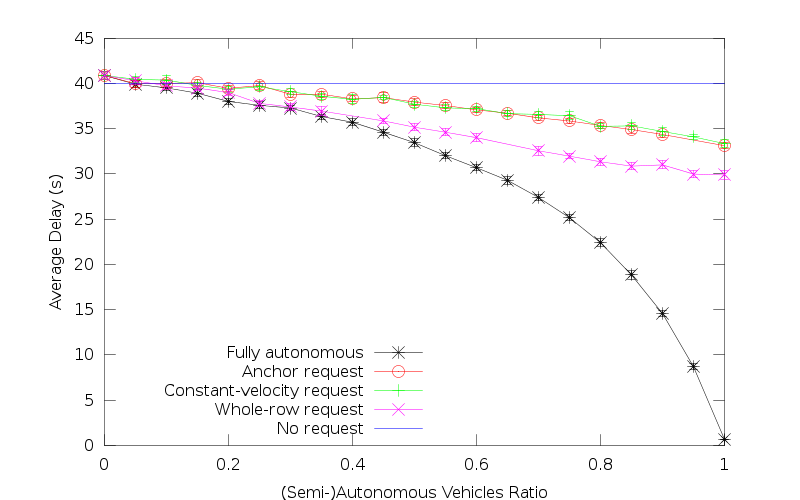
\includegraphics[width=0.8\columnwidth]{figures/figure_2.png}
\caption{(Semi-)Autonomous vehicles vs. Human-Driven vehicles, traffic
level = 360 vehicles/lane/hour. The simulation time is 1800 seconds.
Each data point is an average of the delay times over 30 runs.}
\label{fig:figure2}

\centering
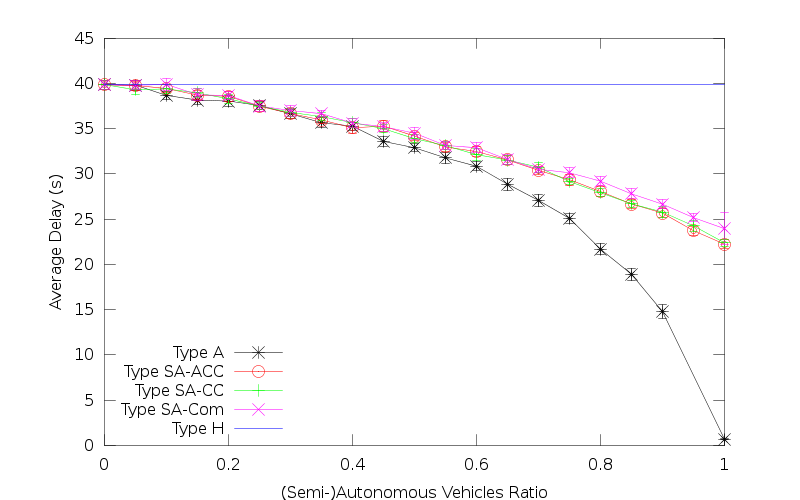
\includegraphics[width=0.8\columnwidth]{figures/figure_1.png}
\caption{Comparison on different features of semi-autonomous vehicles
, traffic level = 360 vehicles/lane/hour. The simulation time is 1800
seconds. Each data point is an average of the delay times over 30 runs.}
\label{fig:figure1}

\mbox{}

\end{figure}

% Figure~\ref{fig:figure1} shows that as the number of autonomous
% vehicles increases, the average delay decreases. In particular, when
% most vehicles are autonomous, the average delay is close to zero.  In
% the second experiment, we created a traffic consisting of
% human-controlled vehicles and two kinds of semi-autonomous vehicles
% but no autonomous vehicles.  We measured the average delay of all
% vehicles when we gradually increased the percentage of semi-autonomous
% vehicles.  Then we compared SemiAIM with optimized traffic signals.
% The results in Figure~\ref{fig:figure2} shows that as the number of
% semi-autonomous vehicles increases, the average delay decreases under
% SemiAIM.  While the decrease is not as dramatic as the decrease when
% the percentage of autonomous vehicles is near 100\% in
% Figure~\ref{fig:figure1}, SemiAIM can reduce about 43\% of the average
% delay when most vehicles are semi-autonomous.

In addition, we compared the performance in traffic with a mixture of
different types of vehicles.  We conducted two experiments to test 1)
the effect of gradually shifting from human-driven vehicles to
autonomous and semi-autonomous vehicles, and 2) the effect of shifting
from semi-autonomous vehicles to fully autonomous vehicles.  The
schedule for shifting is indicated in Tables~\ref{table:3}
and~\ref{table:4}, which can be used to interpret the mix of vehicles
along the x-axes of Figures~\ref{fig:figure3} and~\ref{fig:figure4}
respectively.

\begin{enumerate}

\item Gradually replace human-driven vehicles with semi-autonomous
  vehicles. The result shows that with appearance of more autonomous
  and semi-autonomous vehicles (i.e.\ fewer human-driven vehicles), the
  delay time decreases. The result is shown in
  Figure~\ref{fig:figure3}.

\item Gradually replace semi-autonomous vehicles with fully autonomous
  vehicles. The result shows that when the percentage of human
  vehicles is fixed, the delay time decreases with appearance
  of more autonomous vehicles (i.e.\ fewer semi-autonomous vehicles).
  The result is shown in Figure~\ref{fig:figure4}.

\end{enumerate}

The performance of semi-autonomous vehicles can be significantly
better than human-driven vehicles in small traffic levels. However,
the benefits decrease significantly at higher traffic levels.  In
Figure~\ref{fig:figure5}, we increase the traffic level to 540
vehicles/hour/lane. At this traffic level, congestion appears.  It is
true that semi-autonomy would not ``harm'' normal traffic which
follows traffic signals, but they have almost no chance to enter the
intersection in phases other than when the signal is green. This
condition leads to little or no improvement over traditional traffic
light policy.

This result confirms our hypothesis that while semi-autonomous
vehicles can significantly bridge the gap between the time when all
vehicles are human-driven to that when most are autonomous, there will
likely always remain strong benefits of full autonomy, especially at
high traffic levels.  Nevertheless, for lower levels of traffic, the
benefits of semi-autonomy can be large.

% \commentp{These tables should include a column indicating what point
% on the x-axis each row falls.} \commentn{Added.}

\begin{table}[t]
\caption{The distribution of semi-autonomous vehicles in Figure~\ref{fig:figure3}.}
\label{table:3}
\centering
\begin{tabular}{|c|c|c|}
    \hline
    Type H&  Type SA-* (x-axis)&    Type A\\
    \hline
    90&       9&    1\\
    \hline
    87&     11&    2\\
    \hline
    84&     13&    3\\
    \hline
     ...&   ...&   ...\\
    \hline
         0&     69&  31\\
    \hline
\end{tabular}

\mbox{}

\caption{The distribution of semi-autonomous vehicles in Figure~\ref{fig:figure4}.}
\label{table:4}
\centering
\begin{tabular}{|c|c|c|}
    \hline
     Type H&  Type SA-* (x-axis)&    Type A\\
    \hline
     10&     85&    5\\
    \hline
     10&     80&  10\\
    \hline
     10&     75&  15\\
    \hline
      ...&  ...&  ...\\
    \hline
        10&       5&  85\\
    \hline
\end{tabular}

\end{table}


\begin{figure}
\centering
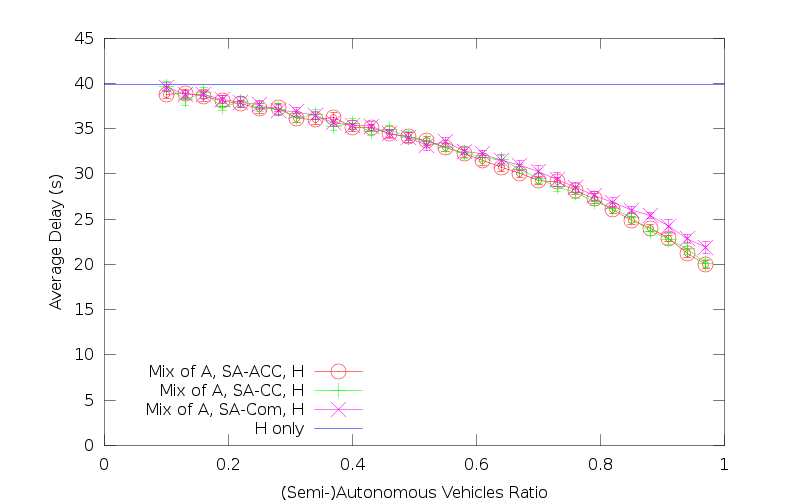
\includegraphics[width=0.8\columnwidth]{figures/figure_3.png}
\caption{The average delay time in different percentage of semi-autonomous
  vehicles and autonomous vehicles. The combination of each point is
  specified in Table \ref{table:3}. Traffic level = 360 vehicles/lane/hour.
  Simulation time is 1800 seconds.}
\label{fig:figure3}

\mbox{}

\centering
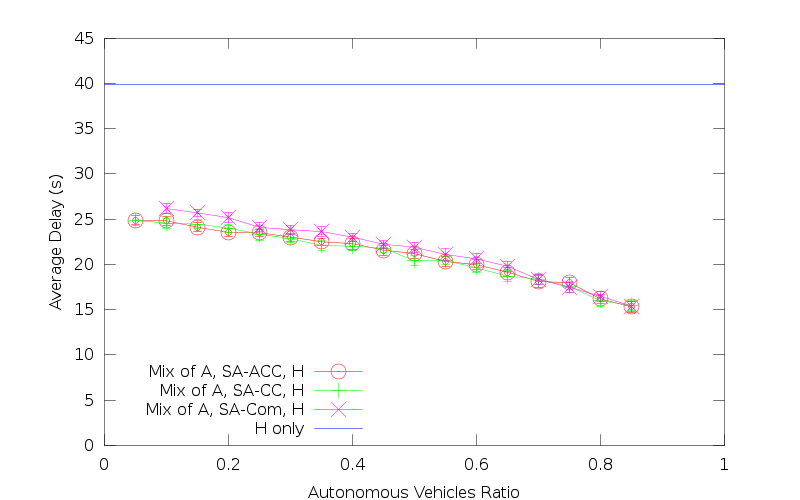
\includegraphics[width=0.8\columnwidth]{figures/figure_4.png}
\caption{The average delay time in different percentage of human
driven vehicles and semi-autonomous vehicles.  The combination of
each point is specified in Table \ref{table:3}.  traffic level = 360
vehicles/lane/hour. Simulation time is 1800 seconds.}
\label{fig:figure4}

\mbox{}

\centering
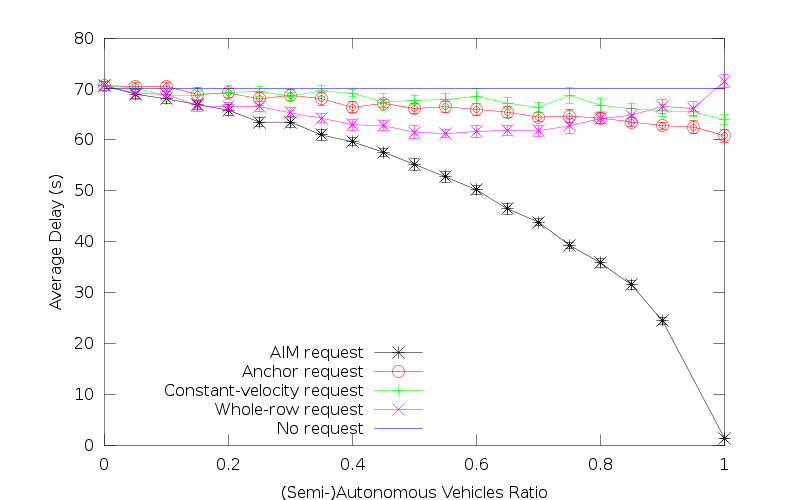
\includegraphics[width=0.8\columnwidth]{figures/figure_5.png}
\caption{Comparison on different features of semi-autonomous vehicles,
traffic level = 540 vehicles/lane/hour. Simulation time is 3600 seconds.}
\label{fig:figure5}
\end{figure}

% \commentp{If we end up with more space to use, it would be good to do
% one or two experiments along the lines of the future work mentioned in
% the last paragraph of the paper. - what happens if there are different
% amounts of traffic in different directions?}
% \commentn{This is mentioned in the future work.}


% To demonstrate the feasibility of SemiAIM as well as evaluate the
% hypothesis that SemiAIM can offer substantial improvements over
% traffic signals and FCFS-Signal, we modified the AIM4 simulator at
% \url{http://www.cs.utexas.edu/~aim} to simulate the behavior of
% vehicles in the constraint-based reservation system and measured the
% average delays of vehicles under (1) AIM, (2) SemiAIM, and (3) traffic
% signals with optimized signal timing.

% \begin{figure}[t]
%   \centering
%   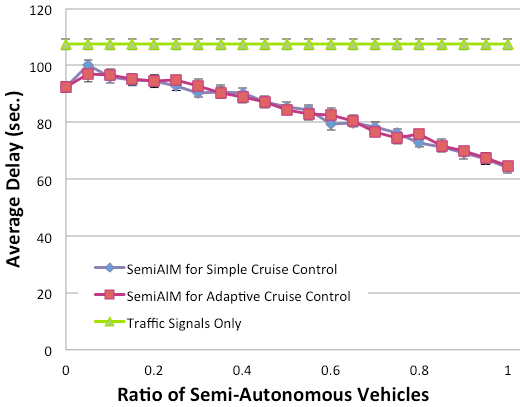
\includegraphics[width=2.4in]{figures/figure2}
%   \caption{Average delay vs. the ratio of semi-autonomous vehicles
% to human-controlled vehicles. T.
%     L. = 720 veh./hour/lane.}
%   \label{fig:figure2}
%   \vspace{-.1in}
% \end{figure}

% The experiments were conducted in a $3 \times 3$ intersection.  In the first
% experiment, the traffic consisted of human-controlled vehicles and
% fully autonomous vehicles only. We gradually increased the percentage
% of autonomous vehicles while keeping the traffic level at 720
% vehicles/hour/lane. We compared two variants of SemiAIM with optimized
% traffic signals in which all vehicles must follow the traffic signals.
% Figure~\ref{fig:figure1} shows that as the number of autonomous
% vehicles increases, the average delay decreases. In particular, when
% most vehicles are autonomous, the average delay is close to zero.  In
% the second experiment, we created a traffic consisting of
% human-controlled vehicles and two kinds of semi-autonomous vehicles
% but no autonomous vehicles.  We measured the average delay of all
% vehicles when we gradually increased the percentage of semi-autonomous
% vehicles.  Then we compared SemiAIM with optimized traffic signals.
% The results in Figure~\ref{fig:figure2} shows that as the number of
% semi-autonomous vehicles increases, the average delay decreases under
% SemiAIM.  While the decrease is not as dramatic as the decrease when
% the percentage of autonomous vehicles is near 100\% in
% Figure~\ref{fig:figure1}, SemiAIM can reduce about 43\% of the average
% delay when most vehicles are semi-autonomous.


% There are four types of
% vehicles in the simulation:
% (1) Human-Controlled Vehicles,
% (2) Semi-Autonomous Vehicles with simple cruise control,
% (3) Semi-Autonomous Vehicles with adaptive cruise control, and
% (4) Fully Autonomous Vehicles.




%%% Local Variables: 
%%% mode: latex
%%% TeX-master: "main"
%%% End:

%\section{Related Work}
\label{sec:related}

The main context of our work is an extension to the FCFS policy
proposed by Dresner and Stone~\cite{bib:Dresner08Multiagent}. Their
experimental results indicated that a mixture of human-driven vehicles
and autonomous vehicles is possible, and leads to better performance
than having all human-driven vehicles, which is the current status
quo.  However, their experiments indicated that the impact of
autonomous vehicles is expected to be relatively small until almost all (90-95\%) of
the vehicles on the road are autonomous.  Our extension to embrace
semi-autonomous vehicles shows significant performance benefits all
along the technology presentation curve.

Our work is similar to the analysis of adaptive cruise control
performance by Jerath and Brennan, who showed that by introducing
adaptive cruise control vehicles into traffic, the vehicles would have
a more \textit{condense} performance, thus increasing the efficiency
of traffic~\cite{bib:Jerath10adaptive}.  When compared to our work,
there are two key differences.  First, we are focusing on the
intersection---a place more critical both from the points of view of
congestion and safety, while the analysis of Jerath and Brennan is
focused on highways.  Second, we study five types of vehicles,
compared to the three types considered by Jerath and Brennan.

Although we are not aware of any other work that is directly concerned
with the interaction of semi-autonomous and autonomous vehicles,
research on vehicular autonomy in general has made significant
progress in recent years.  This was in part due to a series of robotic
car competitions such as the \emph{DARPA Grand
Challenges}~\cite{DARPAGrandChallenge}.  These competitions
accelerated the development of autonomous vehicles to the point where
the technical problem of open-road autonomous driving is considered by
some to be essentially solved~\cite{bib:Dresner08Multiagent}.  When pushed to
extremes, autonomous vehicles can even out-perform many human drivers
in carrying out intricate maneuvers~\cite{Squatriglia2010}. The
non-technical barrier for the adaptation of autonomous vehicles are
largely traffic laws and regulations, though this is also being
overcome~\cite{calo2011-nevada}.

The vast majority of research on autonomous vehicles focuses on how to
ensure they run on existing road infrastructure; there is limited
literature on understanding changes to road infrastructure that can
facilitate vehicular autonomy.  One such project on jointly optimizing
autonomous vehicles and road infrastructure is the PATH program, which
relies on magnetic markers in the roadway for measuring steering angle
and vehicle movements~\cite{bib:Shladover91Automated}.  The Autonomous
Intersection Management~(AIM) protocol~\cite{bib:Dresner08Multiagent, trr11,
bib:Quinlan10Bringing} is a vehicle-to-infrastructure (V2I) mechanism in
which vehicles request space-time in the intersection for their
trajectories prior to arriving at the intersection; a server at the
intersection handles these requests, granting or rejecting
reservations using a grid-based collision detection scheme. This
protocol is enhanced to reduce network traffic and increase safety
using spatial-temporal buffers surrounding the vehicles~\cite{trr11}.

Vehicle-to-Vehicle (V2V) forms of autonomous intersection management
have also been investigated~\cite{naumann97:intersection,
ATT08-vanmiddlesworth}.  In this form, no centralized server is
required (i.e., there is no single point of failure) and vehicles
coordinate in a peer-to-peer fashion when crossing the
intersection. Naumann {\em et al.} investigated a distributed policy
that uses virtual ``tokens'' that a vehicle must possess to cross
certain contested areas of the
intersection~\cite{naumann97:intersection} and formally evaluated it
using petri-nets.  VanMiddlesworth {\em et al.} developed an
AIM-inspired protocol that enables vehicles to ``call ahead'' to
reserve space-time in the
intersection~\cite{ATT08-vanmiddlesworth}. Their protocol outperformed
the traditional stop sign in light traffic. Anchor requests we
introduced in this paper can be implemented using V2V communications.

% We implemented a slightly
% simplified version of the protocol in~\cite{ATT08-vanmiddlesworth}
% that does not use estimated time of arrival and demonstrated that it
% also outperforms a stop sign in light traffic.

Other researchers have investigated autonomous intersections using
real systems involving multiple mobile vehicles.  For example, Kolodko
and Vlacic used golf-cart-like Imara vehicles in evaluating an
autonomous intersection~\cite{Kolodko03:INRIA}.  In their study, all
vehicles must come to a complete stop at the intersection irrespective
of traffic conditions.  Our work differs from this, and all other
previous research by incorporating semi-autonomous vehicles into the
mix, along with autonomous and human-driven cars.



% \section{Related Work}

% The main context of our work is an extension to the FCFS policy
% proposed by Dresner and Stone~\cite{bib:Dresner08Multiagent}. Their
% experimental results indicated that a mixture of human-driven vehicles
% and autonomous vehicles is possible, and leads to better performance
% than having all human-driven vehicles, which is the current status
% quo.  However, their experiments indicated that the impact of
% autonomous vehicles was relatively small until almost all (90-95\%) of
% the vehicles on the road are autonomous.  Our extension to embrace
% semi-autonomous vehicles, shows significant performance benefits all
% along the technology presentation curve.

% Our work is similar to the analysis of adaptive cruise control
% performance by Jerath and Brennan~\cite{bib:Jerath10adaptive}.  Jerath
% and Brennan showed that by introducing adaptive cruise control
% vehicles into traffic, the vehicles would have a more
% \textit{condense} performance, thus increasing the efficiency of
% traffic.  There are two key differences.  First, we are focusing on
% the intersection---a place more critical both from the points of view
% of congestion and safety, while the analysis of Jerath and Brennan is
% focused on highways.  Second, we study five types of vehicles,
% compared to the three types considered by Jerath and Brennan.  




%The
%features of these types of vehicles are various. We are able to see
%which features would increase the efficiency of the intersection the
%most.


% We did not require platooning in our analysis. Vehicles appear randomly
% at the spawning point of each lane. This is also the case for other
% policies that we are going to compare with in this paper.  Our
% analysis is also universal, not restricted to any manufacture. We will
% list the features of each type of semi-autonomous vehicles. Any type
% of cruise control vehicle or adaptive cruise control vehicle that
% satisfy these features can all be applied to the policy mentioned in
% our paper.


%%% Local Variables: 
%%% mode: latex
%%% TeX-master: "main"
%%% End:

\section{Conclusions and Future Work}
\label{sec:conclusions}

This abstract introduces SemiAIM, a new multiagent constraint-based
autonomous intersection management system that enables human-driven
vehicles and semi-autonomous vehicles, in addition to fully autonomous
vehicles, to make reservations and enter an intersection within the
AIM paradigm.  To the best of our knowledge, SemiAIM is the first
multiagent protocol to enable smooth interactions between
human-driven, fully autonomous, and semi-autonomous vehicles.  Our
initial
experiment showed that our system can greatly decrease
traffic delay when most vehicles are semi-autonomous, even when few
(if any) are fully autonomous.

% This study opens up several interesting directions for future work.
% For example, an open question is how to design better constraint-based
% reservation requests using more accurate profiling of the vehicles'
% physical behavior.  It will also be important to study in detail the
% performance of SemiAIM under a variety of different, or varying,
% traffic levels, and with different amounts of traffic traveling in
% different directions.


% the different types of
% constraint-based reservation requests affect the efficiency of
% SemiAIM.  Some reservation requests are much less efficient than the
% others, and how to design 
% efficient reservation requests is an
% important topic for the future.  




% ---not restricted to ones
% described in this paper, but general reservation requests that can be
% understood by the intersection manager---


% \commentp{Isn't that what our experiments already do?  What's
% different here?} \commentn{I think this is what Chiu means..} 


%%% Local Variables: 
%%% mode: latex
%%% TeX-master: "main"
%%% End:


% \bibliographystyle{IEEEtran}
\bibliographystyle{abbrv}
\bibliography{bib/ref,bib/chiu,bib/intelligent_vehicles,bib/intersection,bib/peter}

\end{document}

%%% Local Variables: 
%%% mode: latex
%%% TeX-master: t
%%% End:
